\documentclass{book}

\usepackage{fontspec}
%\newfontfamily\pIqaD{pIqaD-qolqoS.ttf}
\newfontface  \pIqaD{pIqaD-qolqoS.ttf}
%\setmainfont[Ligatures=TeX]{ebgaramond}
\usepackage{ebgaramond}

%\usepackage[utf8]{inputenc}
%\usepackage[T1]{fontenc}
\usepackage[finnish]{babel}
\usepackage[a5paper]{geometry}
\usepackage{dcolumn}
\usepackage{multirow}
\usepackage{amssymb}
\usepackage{makeidx}
\usepackage{longtable}
\usepackage{enumitem}
\usepackage{hyperref}
\usepackage{tikz}

\makeindex

\title{{\pIqaD   }\\Klingonin kielioppi}
\author{Iikka Hauhio}

\setlength{\parindent}{0cm}
\setlength{\parskip}{1em}
\setlist[itemize]{parsep=0pt}
\setlist[enumerate]{parsep=0pt}
\newcolumntype{B}[0]{>{\bfseries}}
\newcolumntype{I}[0]{>{\itshape}}
\newcolumntype{T}[0]{>{\pIqaD}}

\begin{document}

\frontmatter

\maketitle

\newpage
\vspace*{\fill}
1. painos

© 2020 Iikka Hauhio

%\textbf{Osittainen kopiointikielto} \\
%Tämän teoksen kopioiminen on tekijänoikeuslain (404/61, muut. 849/18) mukaisesti kielletty lukuunottamatta Suomen valtion ja Kopiosto r.y.:n tekemässä sopimuksessa tarkemmin määriteltyä osittaista kopiointia opetustarkoituksiin.

\textbf{Kopiointi sallittu} \\
Tämän teoksen kopiointi on sallittu Creative Commons Nimeä 4.0 Kansainvälinen -lisenssin ehdoilla.
Kopiointi, muokkaaminen ja jakaminen on sallittu, mutta alkuperäisen tekijän nimi on ilmoitettava.

http://creativecommons.org/licenses/by/4.0/

\chapter{Alkusanat}

Tämä on yritys soveltaa olemassaolevaa kielitieteen käsitteistöä klingoniin.
Kielen ominaisuudet on kuvattu lyhyesti ja jokaisesta kuvatusta ilmiöstä on joukko esimerkkilauseita.
Tyylillisesti kirja yrittää mukailla lukion oppilaille suunnattuja kielioppeja.

Koska kirja on tarkoitettu myös vasta-alkajille, klingoni on kirjoitettu romanisoiduilla aakkosilla klingonin oman pIqaD-aakkoston sijaan.
Se ei ole oppikirja, vaan sitä on tarkoitus käyttää viiteteoksena muun kurssimateriaalin tukena.

Koska vasta opettelen klingonia kirjoittaessani tätä, tekstissä saattaa olla virheitä.

\begin{quote}
    Iikka Hauhio \\
    \textit{Helsingissä heinäkuussa 2020}
\end{quote}

\chapter{'et mu'}

tlhIngan Hol vIrIchtaHvIS HolQeD mu' tu'lu'bogh vIlo'meH, paqvam vIqonta'.
nom pab vIDel 'ej ghantoH mu'tlheghmey ghaj paq Hoch 'ay'.
patlh cha'DIch DuSaQ jen pab paqmey rur paqvam, 'e' vInID.

ghojwI' chu'vaD paqvam vIqonta'mo', tlhIngan Hol mu'meyvaD roma'ngan ngutlhmey vIlo' 'ej pIqaD vIlo'be'.
ghojmeH paq 'oHbe' paqvam'e'. latlh DuSaQ paqmey Qutlh 'ej pab neH ngaS.

paqvam vIqontaHvIS tlhIngan Hol vIghojtaHmo' neH, chaq Qagh tu'lu'.
net bolu'chugh, HIja'.

\begin{quote}
    'Iyqa' HawHI'o' \\
    \textit{HelsIngqI'Daq, tera' jar Hoch, tera' DIS 2020}
\end{quote}

\tableofcontents

\mainmatter

\chapter{Substantiivit}

\section{Substantiivin suku}
\index{suku}

Klingonin substantiivit jaetaan kolmeen sukuun:

\begin{enumerate}
\item Henkilöt
\item Ruumiinosat
\item Muut sanat
\end{enumerate}

\subsection{Henkilöt}

Ihmiset, klingonit, ihmisiin rinnastettavat tekoälyt, muut älykkäät kieltä käyttävät olennot

\begin{tabular}{Bl Il}
nuv & henkilö \\
puq & lapsi \\
Human & ihminen \\
tera'ngan & maan asukas \\
tlhIngan & klingoni \\
SuvwI' & soturi \\
ghojmoHwI' & opettaja \\
\end{tabular}

\subsection{Ruumiinosat}

Raajat, elimet, muut ruumiinosat (ei ruumis kokonaisuutena)

\begin{tabular}{Bl Il}
ghIch & nenä \\
ghop & käsi \\
tIq & sydän \\
DIr & iho \\
\end{tabular}

Sanat kuuluvat tähän sukuun yleensä vaikka ne olisivat vertauskuvallisia tai alkuperäinen merkitys on muuten etääntynyt.

\begin{tabular}{Bl Il}
    Ho'Du' & sankarit \\
\end{tabular}

\subsection{Muut sanat}

Eläimet, ei-älykkäät elämänmuodot, esineet, asiat, käsitteet

\begin{tabular}{Bl Il}
Duj & alus \\
porgh & vartalo \\
yab & mieli \\
qoq & robotti \\
qaghwI' & '-merkki \\
\end{tabular}

\section{Liitteiden järjestys}

Klingonissa substantiiviliitteiden on aina oltava seuraavalla tavalla järjestyksessä:

\begin{tabular}{l Bl}
juuri & Duj \\
johdin & -Hom \\
täsmennysliite & -qoq \\
monikon tunnnus & -mey \\
omistusliite tai demonstratiiviliite & -lIj \\
sijapääte & -mo' \\
\end{tabular}

\textbf{DujHeyqoqmeylIjmo'} \textit{Sinun niin kutsuttujen pikku alustesi vuoksi}

\section{Johdinliitteet}
\index{-'a'}
\index{-Hom}
\index{-oy}

\begin{tabular}{l Bl | Bl Il}
    augmentatiivi & -'a' & veS'a' & suuri sota \\
    diminutiivi 1 & -Hom & vengHom & kylä (pieni kaupunki) \\
    diminutiivi 2 & -oy & vavoy & isi \\
\end{tabular}

\textbf{-Hom}-liitteellä on halveksiva sävy, ja \textbf{-oy}-liitteellä on hellittelevä sävy.

\section{Täsmennysliitteet}
\index{täsmennysliitteet}
\index{-qoq}
\index{-Hey}
\index{-na'}

Täsmennysliiteellä voi ilmaista, kuinka sopiva käytetty sana puhujan mielestä on.

\begin{tabular}{Bl l}
    -qoq & ''niin kutsuttu'' \\
    -Hey & ''ilmeisesti'': puhuja ei ole varma onko käytetty sana oikea \\
    -na' & ''varmasti'': puhuja on varma käyttämästään sanasta \\
\end{tabular}

Esimerkiksi:

\begin{tabular}{l l}
    luj SuvwI'\textbf{qoq}. & Niin kutsuttu soturi hävisi. \\
    ghojwI'\textbf{Hey} 'oH puq'e'. & Lapsi on ilmeisesti oppilas. \\
    Duj\textbf{na'} vIleghpu'. & Näin varmasti aluksen. \\
\end{tabular}

\section{Monikko}
\index{monikko}
\index{-pu'}
\index{-Du'}
\index{-mey}

Monikon tunnus riippuu suvusta.
Lisäksi joillakin ainesanoilla ei ole monikkomuotoa (kuten \textbf{'Iw} \textit{veri})
ja joillakin epäsäännöllisillä sanoilla käytetään monikkomuodon sijasta erityistä kieliopillisesti yksiköllistä monikkosanaa.

\begin{tabular}{l Bl | Bl Il l}
henkilöt & -pu' & puqpu' & lapset & \\
ruumiinosat & -Du' & tIqDu' & sydämet & \\
muut & -mey & qoqmey & robotit & \\
epäsäännölliset & & ngop & lautaset & (\textbf{jengva'} \textit{lautanen}) \\
\end{tabular}

Jos \textbf{-mey}-liitettä käyttää henkilöiden, ruumiinosien tai epäsäännöllisten sanojen kanssa, sen merkitys on \textit{siellä täällä}:

\begin{tabular}{l l}
    \textbf{puqmey} vIlegh. & Näin lapsia siellä täällä. \\
    qatlh \textbf{jengva'mey} tu'lu'? & Miksi lautasia on siellä täällä? \\
\end{tabular}

\section{Omistusliitteet}
\index{omistusliite}
\index{-wI'}
\index{-wIj}
\index{-ma', -maj}
\index{-lI'}
\index{-lIj}
\index{-ra', -raj}
\index{-Daj}
\index{-chaj}

Omistusliitteet riippuvat monikon tunnuksen tavoin omistettavan asian suvusta.

\begin{tabular}{l Bc Bc}
& \multicolumn{2}{c}{omistettava asia} \\
& \multicolumn{1}{c}{henkilöt} & \multicolumn{1}{c}{muut} \\
minun & -wI' & -wIj \\
sinun & -lI' & -lIj \\
hänen/sen & \multicolumn{2}{Bc}{-Daj} \\
meidän & -ma' & -maj \\
teidän & -ra' & -raj \\
heidän/niiden & \multicolumn{2}{Bc}{-chaj} \\
\end{tabular}

Esimerkiksi:

\begin{tabular}{Bl Il}
tIqwIj & sydämeni \\
puqlI' & lapsesi \\
batlhmaj & kunniamme \\
juHDaj & (hänen) kotinsa \\
\end{tabular}

\section{Demonstratiiviliitteet}
\index{demonstratiiviliite}
\index{-vam}
\index{-vetlh}

Demonstratiiviliitteet osoittavat mistä tai kenestä on kysymys.
Klingon kielessä on kaksi demonstratiiviliitettä:

\begin{tabular}{Bl Il}
    -vam & tämä \\
    -vetlh & tuo \\
\end{tabular}

Demonstratiiviliitettä ja omistusliitettä ei voi käyttää yhtä aikaa.

\begin{tabular}{Bl Il}
    paqvam & tämä kirja \\
    nuvpu'vam & nämä henkilöt \\
    Humanvetlh & tuo ihminen \\
    yabmeyvetlh & nuo mielet \\
\end{tabular}

\section{Sijamuodot}
\index{sijamuodot}

Klingonin kielessä on kuusi sijamuotoa.

\begin{tabular}{l Bl | Bl Il}
nominatiivi & - & Duj & alus \\
lokatiivi & -Daq & DujDaq & aluksessa, alukseen \\
elatiivi & -vo' & Dujvo' & aluksesta \\
datiivi & -vaD & DujvaD & alukselle \\
kausatiivi & -mo' & Dujmo' & aluksen vuoksi \\
aiheellistin & -'e' & Duj'e' & alus \\
\end{tabular}

\subsection{Nominatiivi}
\index{nominatiivi}

Nominatiivia käytetään

1. ilmaisemaan lauseen subjektia ja objektia
\index{subjekti}
\index{objekti}

\begin{tabular}{l l}
    qet \textbf{puqpu'}. & Lapset juoksevat. \\
    \textbf{Soj} vISop. & Syön ruokaa. \\
\end{tabular}

2. ilmaisemaan omistamista

\begin{tabular}{l l}
    \textbf{be'} paq vIlaD. & Luen naisen kirjaa. \\
    tIn \textbf{ghojmoHwI'} ghIch. & Opettajan nenä on suuri. \\
\end{tabular}

3. ilmaisemaan kansalaisuutta

\begin{tabular}{l l}
    Dun \textbf{tlhIngan} wo'. & Klingon-valtakunta on suuremmoinen. \\
\end{tabular}

4. eräissä sanaliitoissa

\begin{tabular}{l Il}
    \textbf{ropyaH} qach & sairaala \\
    \textbf{QIn} 'echletHom & postikortti \\
\end{tabular}

5. postposition edellä
\index{postpositio}

\begin{tabular}{l l}
    \textbf{raS} bIngDaq 'oH tu'lu'. & Se on pöydän alla. \\
\end{tabular}

\subsection{Lokatiivi}
\index{lokatiivi}
\index{-Daq}

Lokatiivia käytetään ilmaisemaan

1. sijaintia

\begin{tabular}{l l}
    reH \textbf{juHwIjDaq} jISop. & Syön aina kotona. \\
\end{tabular}

2. määränpäätä

\begin{tabular}{l l}
    \textbf{juHDaq} yIjaH! & Mene kotiin! \\
    'u' \textbf{HeHDaq} tlhIngan juHqo'vo'. & Klingonien kotimaailmasta \\
    & maailman laidalle. \\
\end{tabular}

\subsection{Elatiivi}
\index{elatiivi}
\index{-vo'}

Elatiivi ilmaisee lähtöpaikkaa.

\begin{tabular}{l l}
    \textbf{yuQvamvo'} jIleng 'e' vIneH. & Haluan matkustaa pois tältä \\
    & planeetalta. \\
    \textbf{nachlIjvo'} mIv yItuQHa'moH! & Riisu kypärä päästäsi! \\
\end{tabular}

\subsection{Datiivi}
\index{datiivi}
\index{-vaD}

Datiivia käytetään

1. ilmaisemaan vastaanottajaa

\begin{tabular}{l l}
    \textbf{SoHvaD} QIn ngeHpu' ghaH. & Hän lähetti sinulle viestin. \\
    \textbf{puqwI'vaD} Soj vIje'. & Ostan ruokaa lapselleni. \\
\end{tabular}

2. ilmaisemaan -moH-verbin kokijaa
\index{-moH}

\begin{tabular}{l l}
    \textbf{ghaHvaD} quHDaj qawmoH. & Se muistuttaa häntä perinnöstään. \\
\end{tabular}

3. pong-verbin kanssa

\begin{tabular}{l l}
    \textbf{vavwI'vaD} ''vavoy'' vIpong. & Kutsun isääni ''vavoyksi''. \\
\end{tabular}

\subsection{Kausatiivi}
\index{kausatiivi}
\index{-mo'}

Kausatiivia käytetään ilmaisemaan syytä

\begin{tabular}{l l}
    \textbf{ropmo'} juHvo' jImejbe'. & En lähde kotoa sairauden takia. \\
\end{tabular}

\subsection{-'e'}
\index{-'e'}

-'e'-sijamuotoa käytetään

1. ilmaisemaan predikatiivilauseen subjektia

\begin{tabular}{l l}
    ghojmoHwI' ghaH \textbf{loDvetlh'e'}. & Tuo mies on opettaja. \\
\end{tabular}

2. lauseenvastikkeissa

\begin{tabular}{l l}
    \textbf{Doch'e'} ghojmoHbogh ghaH Daqaw'a'? & Muistatko, mitä hän \\
    & opetti? \\
\end{tabular}

3. painottamaan lauseen subjektia tai objektia

\begin{tabular}{l l}
    'ut \textbf{Qu''e'}, 'utbe' latlh Doch. & Tehtävä on tärkeä, muut asiat \\
    & eivät. \\
\end{tabular}

4. vertailurakenteessa

\begin{tabular}{l l}
    \textbf{QeD'e'}, HolQeD 'ut law', Hoch 'ut puS. & Kielitiede on tärkein tiede.
\end{tabular}

\chapter{Postpositiot}
\index{postpositio}

Klingonin postpositiot ilmaisevat paikkaa ja taipuvat paikallissijoissa (\textbf{-Daq}, \textbf{-vo'}).
\index{-vo'}
\index{-Daq}

\begin{tabular}{Bl Il | Bl l}
    Dung & yläpuoli & qach DungDaq & rakennuksen yllä/ylle \\
    bIng & alapuoli & raS bIngDaq & pöydän alla/alle \\
    tlhop & etupuoli & Duj tlhopDaq & aluksen edessä/eteen \\
    'em & takapuoli & Dub 'emDaq & selän takana/taakse \\
    nIH & oikea puoli & loD nIHDaq & miehestä oikealla/e \\
    poS & vasen puoli & loD poSDaq & miehestä vasemmalla/e \\
    qoD & sisäpuoli & qach qoDDaq & rakennuksen sisällä/e \\
    Hur & ulkopuoli & Duj HurDaq & ulkona/ulos aluksesta \\
    joj & välitila & qachmey jojDaq & rakennusten välissä/väliin \\
\end{tabular}

\chapter{Verbit}
\index{verbi}

\section{Adjektiivisuus}
\index{adjektiivi}

Klingonin verbit voidaan jakaa transitiivisiin ja intransitiivisiin.
Intransitiivisista verbeistä osa on adjektiivisia ja osa ei.
Adjektiiviset verbit vastaavat muiden kielten adjektiiveja.
\index{transitiivinen verbi}
\index{intransitiivinen verbi}

\begin{tabular}{Bl Il | l l}
    ru' & olla väliaikainen & \textbf{ru'} roj. & Rauha on väliaikainen. \\
    tIn & olla suuri & \textbf{tIn} Dujvam. & Tämä alus on suuri. \\
    mach & olla pieni & \textbf{mach} ghunwI'. & Ohjelmoija on pieni. \\
    'ut & olla tärkeä & \textbf{'ut} Qu'. & Tehtävä on tärkeä. \\
\end{tabular}

Adjektiivinen verbiä voidaan käyttää attribuuttina pääsanansa jälkeen.
Tällöin verbillä voi olla vain päätteet \textbf{-Ha'}, \textbf{-be'} ja \textbf{-qu'}. [Onko varmasti näin?]

\begin{tabular}{l l}
    roj \textbf{ru'} wIneH. & Haluamme väliaikaisen rauhan. \\
    Duj \textbf{tIn} vIghaj. & Minulla on iso alus. \\
    po' \textbf{ghunwI'} mach. & Pieni ohjelmoija on taitava. \\
    Qu' \textbf{'ut} yIqIlQo'! & Älä hylkää tärkeää tehtävää! \\
\end{tabular}

Substantiivin sijamuoto liitetään viimeiseen adjektiiviattribuuttiin, jos sellaisia on.

\begin{tabular}{l l}
    ghunwI'pu' \textbf{machvaD} & Opetan kielitiedettä \\
    HolQeD vIghoHmoH. & pienille ohjelmoijille. \\ 
\end{tabular}

\section{-Ha'-johdin}
\index{-Ha'}

\textbf{-Ha'}-johdin muuttaa verbin merkityksen usein vastakohtaiseksi.
Se liitetään aina verbin juureen.

\begin{tabular}{Bl Il | Bl Il}
    par & inhota & parHa' & tykätä \\
    muS & vihata & musHa' & rakastaa \\
    quv & kunnioittaa & quvHa' & häpäistä \\
    nob & antaa & nobHa' & palauttaa \\
    ru' & olla väliaikainen & ru'Ha' & olla pysyvä \\
\end{tabular}

Joillakin verbeillä johtimen merkitys on \textit{tehdä väärin}.

\begin{tabular}{Bl Il | Bl Il}
    jatlh & puhua & jatlhHa' & sanoa väärin \\
    yaj & ymmärtää & yajHa' & ymmärtää väärin \\
\end{tabular}

\section{Persoona}
\index{persoonamuodot}

Klingonin verbit kongruoivat sekä subjektin että objektin kanssa.
Persoonan tunnus on verbin etuliite.

\begin{tabular}{Bc | Bc | Bc | Bc | Bc | Bc | Bc l}
    \multicolumn{7}{c}{Objekti} & Subjekti \\
    \multicolumn{1}{c}{jIH} & \multicolumn{1}{c}{maH} &\multicolumn{1}{c}{SoH} &\multicolumn{1}{c}{tlhIH} &\multicolumn{1}{c}{ghaH} &\multicolumn{1}{c}{chaH} &\multicolumn{1}{c}{-} & \\
    \multicolumn{1}{c}{} & \multicolumn{1}{c}{} &\multicolumn{1}{c}{} &\multicolumn{1}{c}{} &\multicolumn{1}{c}{'oH} &\multicolumn{1}{c}{bIH} &\multicolumn{1}{c}{} & \\
    - & - & qa- & Sa- & \multicolumn{2}{Bc |}{vI-} & jI- & jIH \\
    \cline{1-7}
    - & - & pI- & re- & wI- & DI- & ma- & maH \\
    \cline{1-7}
    cho- & ju- & - & - & \multicolumn{2}{Bc |}{Da-} & bI- & SoH \\
    \cline{1-7}
    tu- & che- & - & - & \multicolumn{2}{Bc |}{bo-} & Su- & tlhIH \\
    \cline{1-7}
    \multirow{2}{*}{mu-} & \multirow{2}{*}{nu-} & Du- & \multirow{2}{*}{lI-} &$\varnothing$- & \multicolumn{2}{Bc}{\multirow{2}{*}{$\varnothing$-}} & ghaH/'oH \\
    \cline{3-3}
    \cline{5-5}
    & & nI- & & lu- & \multicolumn{2}{c}{} & chaH/bIH \\
    \hline
    vI-lu' & wI-lu' & Da-lu' & bo-lu' & $\varnothing$-lu' & lu-lu' & - & (passiivi) \\
    \hline
    \multirow{2}{*}{HI-} & \multirow{2}{*}{gho-} & - & - & \multirow{2}{*}{yI-} & \multirow{2}{*}{tI-} & yI- & SoH (imp.)\\
    \cline{3-4}
    \cline{7-7}
    & & - & - & & & pe- & tlhIH (imp.)\\
\end{tabular}
\index{imperatiivi}

Refleksiivipäätteen \textbf{-'egh} kanssa käytetään objektitonta persoonaliitettä.
\index{-'egh}

Passiivirakenteessa käytetään \textbf{-lu'}-päätettä ja persoonapääte valitaan siten, että päätteen objekti on yksikön 3. persoona ja subjekti on lauseen objektin persoona. Katso osio~\ref{sec:passiivi}.
\index{-lu'}

\begin{tabular}{l l}
    \textbf{jISop}. & Minä syön. \\
    Soj \textbf{vISoptaH}. & Minä syön ruokaa. \\
    \textbf{qamuS}. & Minä vihaan sinua. \\
    \textbf{bI'IHqu'}. & Olet todella kaunis. \\
    De'wI' \textbf{Dalo''a'} pagh  & Käytätkö sinä tietokonetta vai \\
    \textbf{Dulo''a'} De'wI'? & tietokone sinua? \\
    \textbf{yImej}! & Lähde! \\
    \textbf{tIHoH}! & Tapa heidät! \\
\end{tabular}

Poikkeuksellisesti verbi \textbf{tu'lu'} ei tarvitse persoonaliitettä.
\index{tu'lu'}

\begin{tabular}{l l}
    yotlhDaq puqpu' \textbf{tu'lu' / lutu'lu'}. & Puistossa on lapsia. \\
\end{tabular}

Jos lauseessa on kolmannen persoonan objekti ja ensimmäisen tai toisen persoonan epäsuora objekti, voi verbiin merkitä epäsuoran objektin mukaisen etuliitteen.

\begin{tabular}{l l}
    \textbf{SoHvaD} QIn vIngeH. / & Lähetin sinulle viestin. \\
    QIn \textbf{qangeH}.
\end{tabular}

\section{Päätteiden järjestys}

Verbin päätteiden on aina oltava seuraavassa järjestyksessä:

\begin{tabular}{l l}
    1. & \textbf{-Ha'} \\
    2. & \textbf{-'egh}, \textbf{-chuq} \\
    3. & \textbf{-nIS}, \textbf{-qang}, \textbf{-rup}, \textbf{-beH}, \textbf{-vIp} \\
    4. & \textbf{-choH}, \textbf{-qa'} \\
    5. & \textbf{-moH} \\
    6. & \textbf{-lu'}, \textbf{-laH} \\
    7. & \textbf{-chu'}, \textbf{-bej}, \textbf{-law'}, \textbf{-ba'} \\
    8. & \textbf{-pu'}, \textbf{-ta'}, \textbf{-taH}, \textbf{-lI'} \\
    9. & \textbf{-neS} \\
    10. & \textbf{-Qo'} \\
    11. & \textbf{-DI'}, \textbf{-chugh}, \textbf{-pa'}, \textbf{-vIS}, \textbf{-meH}, \textbf{-mo'}, \textbf{-bogh}, \textbf{-'a'}, \textbf{-jaj}, \textbf{-wI'}, \textbf{-ghach} \\
    12. & (substantiiviliitteet, mikäli edellinen pääte on \textbf{-wI'} tai \textbf{-ghach}) \\
\end{tabular}

\section{Refleksiivisyys}

Refleksiivipäätteellä ilmaistaan, että lauseen subjekti ja objekti ovat samat.
Klingonissa on kaksi refleksiivipäätettä:

\begin{tabular}{Bl Il}
    -'egh & itseään \\
    -chuq & toisiaan \\
\end{tabular}
\index{-'egh}
\index{-chuq}

Refleksiivisellä verbillä ei ole objektia.

\begin{tabular}{l l}
    \textbf{jIlegh'egh}. & Näen itseni. \\
    \textbf{jIghoj'eghmoH}. & Opetan itseäni. \\
    \textbf{muSchuq} chaH. & He vihaavat toisiaan. \\
\end{tabular}

\section{Modaalipäätteet}
\label{sec:modaali}

Modaalipäätteillä ilmaistaan subjektin valmiutta tai tarvetta tehdä asia.

\begin{tabular}{Bl Il | Bl Il}
    -nIS & tarve & -nISbe' & ei tarvitse \\
    -qang & halukas & -qangbe' & haluton \\
    -rup & valmis (henkilöstä) & -rupbe' & ei valmis \\
    -beH & valmis (asiasta) & -beHbe' & ei valmis \\
    -vIp & pelokas & -vIpbe' & peloton \\
\end{tabular}
\index{-nIS}
\index{-qang}
\index{-rup}
\index{-beH}
\index{-vIp}

\begin{tabular}{l l}
    Soj \textbf{vIghunnISmoH}. & Minun on lämmitettävä ruoka. \\
    DaH \textbf{jISopnISbe'}. & Minun ei tarvitse syödä nyt. \\
    \textbf{maSuvqangbe'chu'}. & Emme halua taistella kuolemaan. \\
    \textbf{SuHeghrup'a'}? & Oletteko valmiita kuolemaan? \\
    \textbf{lengbeH} DujwI'. & Alukseni on valmis matkaamaan. \\
    jIHvaD \textbf{bIlujvIp'a'}? & Pelkäätkö hävitä minulle? \\
\end{tabular}

\section{Muutosjohtimet}

Muutospäätteet \textbf{-choH} ja \textbf{-qa'} ilmaisevat muutosta tilassa.

\begin{tabular}{Bl Il}
    -choH & muuttua jonkinlaiseksi, alkaa tehdä \\
    -qa' & uudestaan \\
\end{tabular}
\index{-choH}
\index{-qa'}

Lisättynä adjektiiviseen verbiin \textbf{-choH} tarkoittaa \textit{muuttua jonkinlaiseksi}:

\begin{tabular}{Bl Il | Bl Il}
    ghun & olla lämmin & ghunchoH & lämmetä \\
    rop & olla sairas & ropchoH & sairastua \\
    tIn & olla suuri & tInchoH & kasvaa \\
\end{tabular}

Muihin verbeihin lisättynä \textbf{-choH} tarkoittaa \textit{alkaa tehdä}:

\begin{tabular}{Bl Il | l l}
    Qong & nukkua & \textbf{jIQongchoH}. & Menen nukkumaan. \\
    muS & vihata & \textbf{qamuSchoH}. & Alan vihata sinua. \\
\end{tabular}

\textbf{-qa'} on kuin \textbf{-choH}, mutta ilmaisee, että sama asia on ollut tai tapahtunut aiemminkin.

\begin{tabular}{l l}
    \textbf{jIQongqa'}. & Menen nukkumaan uudestaan. \\
    \textbf{qamuSqa'}. & Alan vihata sinua taas. \\
\end{tabular}

\section{Kausaalijohdin -moH}
\index{-moH}
\index{kausaali}

1. Liitettynä intransitiiviseen verbiin kausaalipääte \textbf{-moH} muuttaa verbin transitiiviseksi.
\index{transitiivinen verbi}
\index{intransitiivinen verbi}

\begin{tabular}{Bl Il | Bl Il}
    ghun & olla lämmin & ghunmoH & lämmittää \\
    rop & olla sairas & ropmoH & sairastuttaa \\
    tIn & olla suuri & tInmoH & suurentaa, kasvattaa \\
    Qong & nukkua & QongmoH & nukuttaa \\
    Hegh & kuolla & HeghmoH & tappaa \\
    chen & saada muoto & chenmoH & luoda, muodostaa \\
\end{tabular}

Intransitiivisen verbin subjektista tulee transitiivisen verbin objekti.

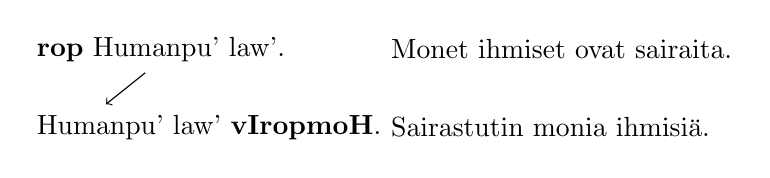
\begin{tikzpicture}
    \node[anchor=west] at (0, 1) {\textbf{rop} Humanpu' law'.};
    \node[anchor=west] at (4.5, 1) {Monet ihmiset ovat sairaita.};
    \draw[->] (1.5, 0.7) -- (1, 0.3);
    \node[anchor=west]  at (0, 0) {Humanpu' law' \textbf{vIropmoH}.};
    \node[anchor=west]  at (4.5, 0) {Sairastutin monia ihmisiä.};
\end{tikzpicture}

2. Liitettynä transitiiviseen verbiin \textbf{-moH} merkitsee ''saada joku tekemään''.

\begin{tabular}{Bl Il | Bl Il}
    ghoj & oppia & ghojmoH & opettaa \\
    ghuH & valmistautua & ghuHmoH & varoittaa \\
    muv & liittyä & muvmoH & rekrytoida \\
    qaw & muistaa & qawmoH & muistuttaa \\
    DoH & perääntyä & DoHmoH & ajaa takaisin \\
\end{tabular}

Alkuperäisen verbin objekti säilyy uuden verbin objektina ja alkuperäisen verbin subjektista tulee uuden verbin epäsuora objekti.

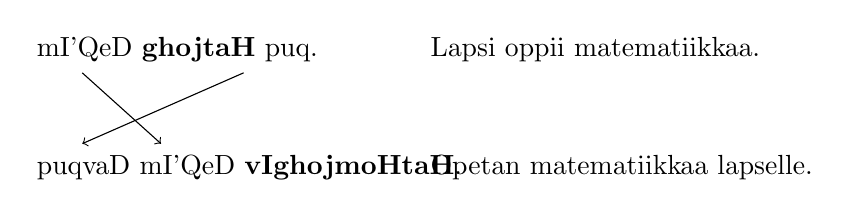
\begin{tikzpicture}
    \node[anchor=west] at (0, 1.5) {mI'QeD \textbf{ghojtaH} puq.};
    \node[anchor=west] at (5, 1.5) {Lapsi oppii matematiikkaa.};
    \draw[->] (2.75, 1.2) -- (0.7, 0.3);
    \draw[->] (0.7, 1.2) -- (1.7, 0.3);
    \node[anchor=west]  at (0, 0) {puqvaD mI'QeD \textbf{vIghojmoHtaH}.};
    \node[anchor=west]  at (5, 0) {Opetan matematiikkaa lapselle.};
\end{tikzpicture}

Jos transitiivisella verbillä on refleksiivipääte, se käyttäytyy kuitenkin samoin, kuin intransitiiviset verbit.

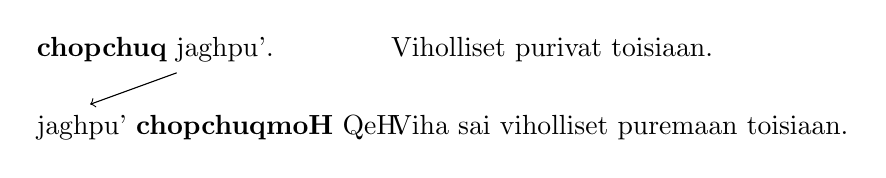
\begin{tikzpicture}
    \node[anchor=west] at (0, 1) {\textbf{chopchuq} jaghpu'.};
    \node[anchor=west] at (4.5, 1) {Viholliset purivat toisiaan.};
    \draw[->] (1.9, 0.7) -- (0.8, 0.3);
    \node[anchor=west]  at (0, 0) {jaghpu' \textbf{chopchuqmoH} QeH.};
    \node[anchor=west]  at (4.5, 0) {Viha sai viholliset puremaan toisiaan.};
\end{tikzpicture}

\section{Passiivisuus}\label{sec:passiivi}
\index{passiivi}
\index{-lu'}

Passiivin tunnus \textbf{-lu'} merkitsee epämääräistä subjektia.
Verbin persoonapääte valitaan kuin objekti olisi subjekti, mutta objekti kirjoitetaan kuintenkin tavanomaisesti ennen predikaattia.
\index{subjekti}
\index{objekti}

\begin{tabular}{l l}
    \textbf{jIqawlu'taH}. & Minut muistetaan. \\
    vay' Daja'chugh, \textbf{bIHoHlu'}. & Jos kerrot jollekulle, sinut tapetaan. \\
    roD juHwIj \textbf{Say'moHlu'}. & Kotini siivotaan säännöllisesti. \\
\end{tabular}

Passiivisessa verbissä ei voi käyttää \textbf{-laH}-päätettä.
\index{-laH}.

\textbf{tu'}-verbin passiivilla on merkitys \textit{olla jossain}:
\index{tu'lu'}

\begin{tabular}{l l}
    raS DungDaq QIn \textbf{tu'lu'}. & Viesti on pöydän päällä. \\
    DeSwarDaq Sut \textbf{tu'lu'be'}. & Kaapissa ei ole vaatteita. \\
\end{tabular}

\section{-laH-pääte}
\label{sec:laH}
\index{-laH}

Modaalinen pääte \textbf{-laH} muuttaa verbin merkitykseksi \textit{voida, osata}.
Se on päätteiden järjestyksessä eri kohdassa kuin muut modaalipäätteet ja sitä ei voi käyttää passiivisissa verbeissä.

\begin{tabular}{Bl Il}
    -laH & voida, osata \\
    -laHbe' & ei voida, ei osata \\
\end{tabular}

Esimerkiksi:

\begin{tabular}{l l}
    tlhIngan Hol \textbf{vIjatlhlaHbe'}. & En osaa puhua klingonia. \\
    \textbf{bIQalnISlaH}. & Sinun on osattava uida. \\
    \textbf{lo'laHghach} ghaj'a'? & Onko sillä arvoa? \\
\end{tabular}

\section{Täsmennyspäätteet}
\label{sec:tasmennys}

Täsmennyspäätteillä ilmaistaan kuinka varma puhuja on ja kuinka selvä kuvattu tilanne on.

\begin{tabular}{Bl Il | Bl Il}
    -chu' & täydellisesti & -chu'be' & epätäydellisesti \\
    -bej & varmasti, kiistatta & -bejbe' & en ole varma \\
    -ba' & selvästi & -ba'be' & ei selvästi \\
    -law' & ilmeisesti & -law'be' & en usko \\
\end{tabular}

\textbf{-chu'} merkitsee, että toiminto suoritetaan täydellisesti, virheettä, oikein. Tarkka merkitys riippuu verbistä.
\index{-chu'}

\begin{tabular}{Bl Il | Bl Il}
    lol & olla ilmassa & lolchu' & olla oikealla korkeudella \\
    nel & sopia & nelchu' & sopia täydellisesti \\
    chuH & heittää keihäs & chuHchu' & osua keihäällä \\
    Suv & taistella & Suvchu' & taistella kuolemaan \\
\end{tabular}

\textbf{-bej} merkitsee, että lause on kiistattomasti tosi.
\index{-bej}

\begin{tabular}{l l}
    \textbf{SuropchoHbej}. & Te sairastutte varmasti. \\
    \textbf{bIlughbejbe'}. & En ole varma, oletko oikeassa. \\
\end{tabular}

\textbf{-ba'} merkitsee, että lauseen uskotaan olevan selvästi tosi, mutta se ei ole yhtä kiistatonta kuin \textbf{-bej}-päätteen kanssa.
\index{-ba'}

\begin{tabular}{l l}
    \textbf{ropba'} ghaH. & Hän on selvästi sairas. \\
    \textbf{bIlughba'be'}. & Ei ole selvää, että olet oikeassa. \\
    \textbf{bIlughbe'ba'}. & Olet selvästi väärässä. \\
\end{tabular}

\textbf{-law'} merkitsee \textit{uskoa, luulla}:
\index{-law'}

\begin{tabular}{l l}
    \textbf{yIropqa'law'}. & Taidan sairastua uudestaan. \\
    \textbf{bIlughlaw'}. & Luulen, että olet oikeassa. \\
    \textbf{bIlughlaw'be'}. & En usko, että olet oikeassa. \\
    \textbf{bIlughbe'law'}. & Luulen, että olet väärässä. \\
\end{tabular}

\section{Aspekti}

Verbin aspekti ja teelisyys voidaan ilmaista tarvittaessa seuraavilla päätteillä:
\index{aspekti}
\index{teelisyys}

\begin{tabular}{l l l}
    & \multicolumn{2}{c}{aspekti} \\
    & imperfektiivinen & perfektiivinen \\
    yleinen & \textbf{-taH} & \textbf{-pu'} \\
    teelinen & \textbf{-lI'} & \textbf{-ta'} \\
\end{tabular}
\index{-taH}
\index{-lI'}
\index{-pu'}
\index{-ta'}
\index{imperfektiivisyys}
\index{perfektiivisyys}
\index{teelisyys}

Imperfektiivisyydellä ilmaistaan, että toiminta on jatkuvaa ja päättymätöntä. 
Perfektiivinen toiminta taas on valmis ja päättynyt.
Aspektia ei tule sekoittaa aikamuotoihin, joita ei ole klingonissa.

Teelisyydellä ilmaistaan, onko toiminnalla tarkoitusta tai määränpäätä.
Pääte \textbf{-lI'} merkitsee, että toiminnalla on määränpää tai tavoite (toiminnan ei tarvitse kuitenkaan olla tahallista).
Pääte \textbf{-ta'} merkitsee, että toiminta on tahallista.
On aina sallittua käyttää teelisten päätteiden sijasta yleisiä päätteitä.

\begin{tabular}{l l}
    \textbf{jISoptaHvIS} yISujQo'. & Älä häiritse minua, kun syön. \\
    \textbf{HeghlI'} ghaH. & Hän on kuolemassa. \\
    qatlh \textbf{DaHoHpu'}? & Miksi tapoit hänet? \\
    \textbf{vIghorta'}. & Rikoin sen tarkoituksella. \\
\end{tabular}

\section{-neS-pääte}

\textbf{-neS}-pääte ilmaisee kunnioitusta keskustelun toista osapuolta kohtaan.
Sitä tulee käyttää vain puhuteltaessa ylempiarvoista henkilöä formaalisti.

\textbf{-neSbe'}-päätettä ei ole sopiva käyttää.

\section{Seikkailijat}

Seikkalijat muuttavat niitä edeltävän morfeemin merkitystä.
\index{seikkalija}

\begin{tabular}{Bl Il}
    -qu' & erittäin \\
    -be' & ei \\
\end{tabular}
\index{-qu'}
\index{-be'}

Modaalipäätteitä ja täsmennyspäätteitä käsittelevissä luvuissa \ref{sec:modaali}, \ref{sec:laH} ja \ref{sec:tasmennys} on selitetty \textbf{-be'}-päätteen vaikutus näihin päätteisiin.
Muussa tapauksessa \textbf{-be'} kiinnitetään yleensä joko verbin juureen, \textbf{-Ha'}-, \textbf{-choH}-, \textbf{-qa'}-, \textbf{-moH}-, \textbf{-lu'}-päätteeseen tai aspektin päätteeseen riippuen siitä, mikä näistä on viimeinen.

Käskymuotoisissa verbeissä käytetään \textbf{-Qo'}-päätettä \textbf{-be'}-päätteen sijasta.
Jos lauseessa on kielteinen sana, kuten \textbf{pagh}, \textbf{not} tai \textbf{wej}, kieltopäätettä \textbf{be'} ei käytetä.

\textbf{-qu'}-pääte voidaan kiinnittää mihin tahansa morfeemiin lukuunottamatta persoonapäätettä ja myöhemmin tässä luvussa esiteltyjä päätteitä, eli jussiivin, interrogatiivin tai partisiipin tunnusta, konjunktiopäätettä tai substantiivijohdinta.

\begin{tabular}{l l}
    \textbf{jIropqu'}! & Olen hyvin sairas! \\
    loD \textbf{'IHqu'} vIlegh. & Näin kauniin miehen. \\
\end{tabular}

\section{-Qo'-pääte}
\index{-Qo'}

1. \textbf{-Qo'}-päätteellä ilmaistaan kieltäytymistä.

\begin{tabular}{l l}
    De'wI' Quj \textbf{vIQujQo'}! & En pelaa tietokonepelejä! \\
    Soj tlhol \textbf{SopQo'} puqwI'. & Lapseni ei suostu syömään raakaa \\
    & lihaa. \\
\end{tabular}

2. Imperatiiviverbiin liitettynä \textbf{-Qo'} merkitsee \textit{älä}.
\index{imperatiivi}

\begin{tabular}{l l}
    \textbf{peqetQo'}! & Älkää juosko! \\
    \textbf{HIquvHa'Qo'}. & Älä häpäiskö minua! \\
\end{tabular}

\section{Jussiivi}

Jussiivin tunnus \textbf{-jaj} ilmaisee toivetta tai kehoitusta.

\begin{tabular}{l l}
    \textbf{taHjaj} tlhIngan wo'! & Eläköön klingonien valtakunta! \\
\end{tabular}

\section{Interrogatiivi}
\index{interrogatiivi}

Interrogatiivi eli kysymysmuoto muuttaa lauseen kysymykseksi.
Interrogatiivin tunnus on \textbf{-'a'}.
\index{-'a'}

\begin{tabular}{l l}
    nIm Datlhutlh\textbf{'a'}? & Juotko maitoa? \\
    tlhIngan Hol Dajatlh\textbf{'a'}? & Puhutko klingonia? \\
\end{tabular}

Interrogatiivia ei käytetä, jos lauseessa on kysymyssana.

\begin{tabular}{l l}
    \textbf{nuq} Datlhutlh? & Mitä juot? \\
    \textbf{qatlh} tlhIngan Hol Dajatlh? & Miksi puhut klingonia? \\
\end{tabular}

\section{Konjunktiopäätteet}
\index{konjunktiopääte}

Konjunktiopäätteet kiinnitetään sivulauseen predikaattiin.

\begin{tabular}{Bl Il}
    -vIS & kun \\
    -DI' & heti kun \\
    -pa' & ennen kun \\
    -chugh & jos \\
    -mo' & koska \\
    -meH & jotta \\
\end{tabular}
\index{-vIS}
\index{-DI'}
\index{-pa'}
\index{-chugh}
\index{-mo'}
\index{-meH}

\textbf{-vIS}-päätteen kanssa on käytettävä imperfektiivistä aspektia (\textbf{-taH}, \textbf{-lI'}).

\begin{tabular}{l l}
    bIropchoH\textbf{chugh}, jImej. & Lähden, jos sairastut. \\
    bItuSchoH\textbf{DI'}, jIqet. & Juoksen heti kun alat yskimään. \\
    jIqettaH\textbf{vIS}, 'oy' 'uSDu'wIj. & Jalkoihini sattuu, kun juoksen. \\
    jIHoSmoH\textbf{meH}, jISuv. & Taistelen voimistuakseni. \\
    bIQob\textbf{mo'}, yIngab! & Koska olet vaarallinen, katoa! \\
    bIchegh\textbf{pa'}, yIQub! & Mieti ennen kun palaat! \\
\end{tabular}

\textbf{-meH}-päätteinen verbi voi määrittää lauseen lisäksi myös substantiivia.

\begin{tabular}{l l Il}
    \textbf{DIlmeH} Huch & ''raha maksamiseen'' & hinta \\
    \textbf{ghojmeH} paq & ''kirja oppimiseen'' & oppikirja \\
    \textbf{HIjmeH} chaw' & ''lupa toimittamiseen'' & postimerkki \\
    \textbf{ngongmeH} Duj & ''alus testaamiseen'' & koealus \\
\end{tabular}

\textbf{-meH}-päätettä käytetään sanan \textbf{Qu'} \textit{tehtävä} kanssa, kun lauseen halutaan olevan toisen lauseen subjekti.

\begin{tabular}{l l}
    Qatlh jagh leghmeH \textbf{Qu'}. & Vihollisen näkeminen on vaikeaa. \\
    jIHvaD potlh SuvmeH \textbf{Qu'}. & Taisteleminen on minulle tärkeää. \\
\end{tabular}

\section{Partisiipit}
\index{partisiippi}

Partisiippi muodostetaan verbistä \textbf{-bogh}-päätteellä.
Partisiippi ei ole adjektiivi, vaan se sijoitetaan joko ennen tai jälkeen pääsanaansa riippuen siitä, onko pääsana verbin subjekti vai objekti.
\index{-bogh}

Aktiivin partisiippi sijoitetaan ennen pääsanaansa.
Tällöin pääsana on partisiipin subjekti.
Passiivin partisiippi taas sijoitetaan pääsanansa jälkeen, jolloin pääsana on partisiipin objekti.

\begin{tabular}{l l}
    \textbf{Qapbogh} SuvwI' & onnistunut soturi \\
    SuvwI' \textbf{jeybogh} & voitettu soturi \\
\end{tabular}

Partisiipilla voi olla sekä subjekti tai objekti.
Jos pääsana on partisiipin objekti, sen on oltava \textbf{-'e'}-sijassa.
Jos taas pääsana on partisiipin subjekti, se voi olla \textbf{-'e'}-sijassa.

\begin{tabular}{l l}
    jagh \textbf{jeybogh} SuvwI' / SuvwI''e' & vihollisen voittanut soturi \\
    SuvwI''e' \textbf{jeybogh} jagh & vihollisen voittama soturi \\
\end{tabular}

\section{Substantiivijohtimet}
\index{substantiivijohdin}

\textbf{-wI'}-johdin vastaa suomen \textit{-ja}-johdinta.
Se muuttaa verbin subjektia vastaavaksi substantiiviksi.
\index{-wI'}

\begin{tabular}{Bl Il | Bl Il}
    ghoj & oppia & ghojwI' & oppilas \\
    ghojmoH & opettaa & ghojmoHwI' & opettaja \\
    nep & valehdella & nepwI' & valehtelija \\
    chIS & olla valkoinen & chISwI' & valkoinen \\
    po' & olla taitava & po'wI' & asiantuntija \\
    ngaQHa'moH & poistaa lukitus & ngaQHa'moHwI' & avain \\
\end{tabular}

\textbf{-ghach}-johdin muuttaa verbin abstraktiksi substantiiviksi.
\index{-ghach}

\begin{tabular}{Bl Il | Bl Il}
    lo'laH & voida käyttää & lo'laHghach & arvo \\
    quvHa' & olla häpäisty & quvHa'ghach & häpeä \\
    bomlaH & voida laulaa & bomlaHghach & laulutaito \\
    wovtaH & olla kirkas & wovtaHghach & kirkkaus \\
    nIv & olla suuremmoinen & nIvghach & suuremmoisuus \\
\end{tabular}

Ei ole selvää, milloin \textbf{-ghach}-johdinta tarvitaan, sillä monet verbit sellaisenaan ovat substantiiveja ilman johdinta.

\begin{tabular}{Bl Il | Bl Il}
    quv & kunnioittaa & quv & kunnia \\
    bom & laulaa & bom & laulu \\
    bel & nauttia & bel & nautinto \\
\end{tabular}

\section{Apuverbit}

\subsection{neH}
\index{neH}

Apuverbin \textbf{neH} \textit{haluta} kanssa ei käytetä relatiivipronominia \textbf{'e'}.

\begin{tabular}{l l}
    jISuv \textbf{vIneH}! & Haluan taistella! \\
\end{tabular}

\subsection{qa'}
\index{qa'}

Apuverbiä \textbf{qa'} \textit{korvata} käytetään \textit{jonkin sijasta} -rakenteessa. Relatiivipronomini \textbf{'e'} on valinnainen.

\begin{tabular}{l l}
    vIghro' vISuqnIS. yIH \textbf{qa'}. & Minun on hankittava kissa tribblen tilalle. \\
    juHDaq jIba'. jIqet ('e') \textbf{qa'}. & Istun kotona juoksemisen sijaan. \\
\end{tabular}

\chapter{Pronominit}

\section{Persoonapronominit}
\index{persoonapronomini}
\index{jIH}
\index{maH}
\index{SoH}
\index{tlhIH}
\index{ghaH}
\index{chaH}
\index{'oH}
\index{bIH}

Klingonissa on seuraavat persoonapronominit:

\begin{tabular}{l Bc Bc}
    persoona & \multicolumn{1}{c}{yksikkö} & \multicolumn{1}{c}{monikko} \\
    1. & jIH & maH \\
    2. & SoH & tlhIH \\
    3., henkilöt & ghaH & chaH \\
    3., muut & 'oH & bIH \\
\end{tabular}

Pronominit toimivat substantiivin tavoin ja niitä voi taivuttaa sijamuodoissa.
Pronomineja ei kuitenkaan voi käyttää ilmaisemaan omistamista, vaan siihen käytetään erillisiä omistusliitteitä.

\begin{tabular}{l l}
    \textbf{ghaH} yIQaH! & Auta häntä! \\
    \textbf{jIHvaD} 'oH yInobHa'. & Palauta se minulle. \\
\end{tabular}

Persoonapronomini voi toimia verbinä, jolloin sen merkitys on \textit{olla}.
Tällöin pronomini voi ottaa verbipäätteitä, mutta ei persoonaetuliitettä.
\index{olla-verbi}

\begin{tabular}{l l}
    tlhIngan \textbf{jIHbe'}. & En ole klingoni.\\
    'Iv \textbf{maH}? & Keitä me olemme? \\
\end{tabular}

\section{Interrogatiivipronominit}
\index{interrogatiivipronomini}
\index{nuq}
\index{'Iv}

Interrogatiivipronominit ovat kysymyssanoina toimivia pronomineja.

\begin{tabular}{Bl Il}
    nuq & mikä \\
    'Iv & kuka \\
\end{tabular}

\textbf{'Iv}-pronominia käytetään henkilöiden kanssa ja \textbf{nuq}-proniminia muiden sanojen kanssa.

Esimerkiksi:

\begin{tabular}{l l}
    DughIj \textbf{nuq}? & Mikä pelottaa sinua? \\
    lugh \textbf{'Iv}? & Kuka on oikeassa? \\
\end{tabular}

Kuten persoonapronominitkin, interrogatiivipronominit voivat toimia verbinä ja niitä voi taivuttaa sijamuodoissa.

\begin{tabular}{l l}
    ghojmoHwI'lI' \textbf{'Iv}? & Kuka on opettajasi? \\
    \textbf{'IvvaD} DangeH? & Kenelle lähetät sen? \\
    \textbf{nuqDaq} bIjaH? & Minne menet? \\
\end{tabular}

\section{Indefiniittipronominit}

\subsection{Kvanttoripronominit}
\index{kvanttoripronomini}
\index{pagh}
\index{vay'}
\index{'op}
\index{Hoch}

Klingonissa on seuraavat kvanttoripronominit:

\begin{tabular}{Bl l}
    pagh & \textit{ei kukaan, ei mikään} \\
    vay' & \textit{joku, jokin} \\
    'op & (laskettaville sanoille:) \textit{jotkut}; (ainesanoille:) \textit{vähän, jonkin verran} \\
    Hoch & \textit{jokainen, kaikki} \\
\end{tabular}

Esimerkiksi:

\begin{tabular}{l l}
    ropchoH, neH \textbf{pagh}. & Kukaan ei halua sairastua. \\
    tlhoy Sop \textbf{vay'}. & Joku söi liikaa. \\
    ru' \textbf{Hoch}. & Kaikki on väliaikaista. \\
\end{tabular}

\textbf{pagh} ja \textbf{Hoch} voivat toimia substantiivin määreinä. \textbf{'op} esiintyy vain substantiivin määreenä.

\begin{tabular}{l l}
    'oH Sov \textbf{Hoch} tlhIngan. & Sen tietää jokainen klingoni. \\
    mutlhej \textbf{pagh} jatlhwI'. & Minulla ei ole ketään kelle puhua. \\
    \textbf{'op} HIq vItlhutlh neH! & Minä vain join vähän viiniä! \\
    mupar \textbf{'op} Qel. & Jotkut lääkärit vihaavat minua. \\
\end{tabular}

\subsection{Pronomini latlh}
\index{latlh}

Indefiniittipronomini \textbf{latlh} merkitsee \textit{toinen}.
\index{indefiniittipronomini}

\section{Relatiivipronominit}
\index{relatiivipronomini}
\index{'e'}
\index{net}

Klingonissa on kaksi relatiivipronominia: \textbf{'e'} ja \textbf{net}.
Molemmat viittaavat edeltävään lauseeseen.

\textbf{'e'} merkitsee \textit{se, että}.

\begin{tabular}{l l}
    Qatlh veS, \textbf{'e'} vISov. & Tiedän, että sota on vaikeaa. \\
    bISuv \textbf{'e'} lulegh. & He näkevät, että olet taistelet. \\
    vaj yInlu' \textbf{'e'} toblu'. & Niin todistaa, että elää. \\
\end{tabular}

\textbf{net} muuttaa lauseen merkityksen passiiviseksi.

\begin{tabular}{l l}
    Qatlh veS, \textbf{net} Sov. & Tiedetään, sota on vaikeaa. \\
    bISuv \textbf{net} legh. & Taistelemisesi nähdään. \\
    yInlu' \textbf{net} tob. & Todistetaan elämistä. \\
\end{tabular}

\textbf{'e'}-pronominia ei käytetä \textbf{neH}-apuverbin kanssa.
\index{neH}

\begin{tabular}{l l}
    jIropHa'choH \textbf{vIneH}. & Haluan parantua. \\
    ghorgh bIQongchoH \textbf{DaneH?} & Milloin haluat mennä nukkumaan? \\
\end{tabular}

\chapter{Adverbit}
\index{adverbi}

Lista yleisimmistä adverbeista on liitteessä~\ref{apx:adverbit}.

\section{Adverbien sijainti}

Yleensä adverbit sijoitetaan lauseen alkuun.

\begin{tabular}{l l}
    \textbf{nom} jIqet. & Juoksen nopeasti. \\
    \textbf{wa'leS} ghaH vIlegh. & Näin hänet eilen. \\
    \textbf{chaq} jIlughbe'. & Ehkä olen väärässä. \\
    \textbf{qatlh} DaHoH? & Miksi tapoit hänet? \\
\end{tabular}

\section{Adverbit je ja neH}
\index{je}
\index{neH}

Poikkeuksellisesti adverbit \textbf{je} \textit{myös}, \textbf{neH} \textit{vain} sijoitetaan predikaatin jälkeen.

\begin{tabular}{l l}
    bIropchoH \textbf{je} vIneHbe'! & En halua, että lisäksi sairastut! \\
    ghaHvaD vIjatlhlaHchugh \textbf{neH}... & Jos vain voisin puhua hänelle... \\
\end{tabular}

\textbf{je} ja \textbf{neH} voivat toimia myös adjektiivin tavoin substantiivin tai pronominin määreinä.

\begin{tabular}{l l}
    tlhIngan Hol \textbf{je} vIjatlh. & Puhun myös klingonia. \\
    Soj tlhol \textbf{neH} vISop. & Syön vain raakaa ruokaa. \\
\end{tabular}

%\section{Adverbi jay'}
% Tämä on kirosana, joten kuuluuko sitä käsitellä "lukion" kielioppikirjassa?

\section{Adverbit law' ja puS}
\index{law'}
\index{puS}

Adverbeja \textbf{law'} \textit{paljon} ja \textbf{puS} \textit{vähän} käytetään vertailurakenteissa.
\index{vertailurakenne}

\begin{tabular}{l l}
    jIH HoS \textbf{law'}, SoH HoS \textbf{puS}. & Olen sinua voimakkaampi. \\
    ghaH po' \textbf{law'be'}, jIH po' \textbf{puSbe'}. & Hän ei ole minua taitavampi. \\
\end{tabular}

Superlatiivirakenteessa käytetään sanaa \textbf{Hoch} \textit{kaikki}.
\index{superlatiivi}
\index{Hoch}

\begin{tabular}{l l}
    ghaH mIp \textbf{law'}, \textbf{Hoch} mIp \textbf{puS}. & Hän on rikkain. \\
    %Duj'e', 'oH wagh \textbf{law'}, \textbf{Hoch} wagh \textbf{puS}. & Se on kallein alus. \\
\end{tabular}

\section{Paikka-adverbeja}
\index{paikka-adverbi}
\index{Dat}
\index{vogh}
\index{naDev}
\index{pa'}

Substantiiveja \textbf{Dat} \textit{kaikkialla}, \textbf{vogh} \textit{jossain}, \textbf{naDev} \textit{täällä} ja \textbf{pa'} \textit{siellä} ei voi taivuttaa lokatiivissa.
Sen sijasta ne toimivat sellaisenaan adverbeina.

\begin{tabular}{Bl Il | r Bl Il l}
    Dat & kaikkialla & ( & Datvo' & kaikkialta & ) \\
    vogh & jossain & ( & voghvo' & jostain & ) \\
    naDev & täällä & ( & naDevvo' & täältä & ) \\
    pa' & siellä & ( & pa'vo' & sieltä & ) \\
\end{tabular}

Sanalla \textbf{pa'} on myös merkitys \textit{huone}.
Tällöin se taipuu normaalisti lokatiivissa.

\begin{tabular}{l l}
    \textbf{pa'} vIQong. & Nukuin siellä. \\
    \textbf{pa'Daq} vIQong. & Nukuin huoneessa. \\
\end{tabular}

\section{Laskuriadverbit}
\index{laskuriadverbi}
\index{leS}
\index{Hu'}
\index{wen}
\index{waQ}
\index{ben}
\index{nem}
\index{ret}
\index{pIq}

Laskuriadverbit seuraavat lukumäärää ja ilmaisevat ajan kulumista.

\begin{tabular}{Bl Il}
    Hu' & päivää sitten \\
    leS & päivän päästä \\
    wen & kuukautta sitten \\
    waQ & kuukauden päästä \\
    ben & vuotta sitten \\
    nem & vuoden päästä \\
    ret & (ajanyksikköä) sitten \\
    pIq & (ajanyksikön) päästä \\
\end{tabular}

Esimerkkejä:

\begin{tabular}{l l}
    cha'maH \textbf{ben} jIbogh. & Olen kaksikymmentä vuotta vanha. \\
    wa'\textbf{leS} jISuvbe'. & En taistellut eilen. \\
    wej \textbf{wen} bIropchoH. & Sairastuit kolme kuukautta sitten. \\
    wa' \textbf{nem} mamIp. & Vuoden päästä olemme rikkaita. \\
\end{tabular}

\textbf{ret} ja \textbf{pIq} seuraavat lukumäärää ja yksikköä.

\begin{tabular}{l l}
    cha' \textbf{rep ret} Hegh. & Hän kuoli kaksi tuntia sitten. \\
    wa'maH \textbf{lup pIq} maHIv. & Hyökkäämme kymmenen sekunnin kuluttua. \\
\end{tabular}

\section{Interrogatiiviadverbit}
\index{chay'}
\index{ghorgh}
\index{qatlh}
\index{'ar}
\index{'arlogh}

\begin{tabular}{Bl Il}
    chay' & miten \\
    ghorgh & milloin \\
    qatlh & miksi \\
    'ar & kuinka monta / paljon \\
    'arlogh & kuinka monta kertaa \\
\end{tabular}

\chapter{Konjunktiot}

\section{'ej, qoj, pagh}
\index{'ej}
\index{qoj}
\index{pagh}

Seuraavat konjunktiot erottavat lauseita, partisiippeja ja adverbeja toisistaan.

\begin{tabular}{Bl Il}
    'ej & ja \\
    qoj & ja/tai \\
    pagh & joko ... tai \\
\end{tabular}

Esimerkiksi:

\begin{tabular}{l l}
    Sopbe' \textbf{'ej} tlhutlhbe' qoqmey. & Robotit eivät syö eivätkä juo. \\
    HoSbogh \textbf{'ej} Qupbogh SuvwI' yoH & rohkea, voimakas ja nuori soturi \\
    taH \textbf{pagh} taHbe'. & Ollako vai eikö olla. \\
\end{tabular}

\section{je, joq, ghap}
\index{je}
\index{joq}
\index{ghap}

Nämä konjunktiot erottavat substantiivilausekkeista toisistaan.

\begin{tabular}{Bl Il}
    je & ja \\
    joq & ja/tai \\
    ghap & joko ... tai \\
\end{tabular}

Esimerkiksi:

\begin{tabular}{l l}
    juHqo' miDmey \textbf{je} wIHub. & Puolustamme kotimaailmaa ja siirtokuntia. \\
\end{tabular}

\textbf{je} merkitsee \textit{myös}, jos sitä edeltää vain yksi substantiivilauseke.

\chapter{Numeraalit}
\index{numeraali}

Klingonin lukusanat muodostetaan kymmenjärjestelmän numeroista ja suuruusluokkaa kuvaavista liitteistä.
\index{lukusana}

\begin{tabular}{Bl Il | Bl Il}
    pagh & nolla & -maH & kymmenen \\
    wa' & yksi & -vatlh & sata \\
    cha' & kaksi & -SaD/-SanID & tuhat \\
    wej & kolme & -netlh & kymmenen tuhatta \\
    loS & neljä & -bIp & sata tuhatta \\
    vagh & viisi & -'uy' & miljoona \\
    jav & kuusi & & \\
    Soch & seitsemän & & \\
    chorgh & kahdeksan & & \\
    Hut & yhdeksän & & \\
\end{tabular}
\index{-maH}
\index{-vatlh}
\index{-SaD}
\index{-SanID}
\index{-netlh}
\index{-bIp}
\index{-'uy'}

Luku esitetään merkitsevin numero ensin kuten suomessakin.
Sanaa \textbf{pagh} \textit{nolla} käytetään vain yksin eikä siihen saa liittää suurusluokkaliitteitä.
\index{pagh}

Esimerkiksi luku 103 621 esitetään seuraavasti:

\begin{tabular}{c c c c c c}
    \textbf{wa'bIp} & & \textbf{wejSaD} & \textbf{javvatlh} & \textbf{cha'maH} & \textbf{wa'} \\
    1 & 0 & 3 & 6 & 2 & 1 \\
    \multicolumn{6}{c}{satakolmetuhattakuusisataakaksikymmentäyksi} \\
\end{tabular}

Luku kirjoitetaan yleensä ennen pääsanaansa.

\begin{tabular}{l l}
    \textbf{cha'} SuvwIpu' & kaksi soturia \\
    Hoch rewbe' QaH \textbf{wa'} mang. & Yksi sotilas auttaa kaikkia \\
    & kansalaisia. \\
\end{tabular}

Luvusta voi tehdä järjestysluvun \textbf{-DIch}-johtimella.
Järjestysluvut kirjoitetaan adjektiivin tavoin pääsanansa jälkeen.
\index{-DIch}
\index{järjestysluku}

\begin{tabular}{l l}
    \textbf{wa'DIch} & \textit{ensimmäinen} \\
    \textbf{cha'DIch} & \textit{toinen} \\
    \textbf{wa'maHDich} & \textit{kymmenes} \\
    veng \textbf{wa'Dich} & Ensimmäinen Kaupunki \\
    \textbf{wa'DIch} jISop. & Syön ensin. \\
\end{tabular}

\textbf{-logh}-johdin muuttaa luvun adverbiksi, jolla on merkitys \textit{kertaa}.
\index{-logh}

\begin{tabular}{Bl Il}
    paghlogh & ei kertaakaan \\
    wa'logh & kerran \\
    cha'logh & kahdesti, kaksi kertaa \\
\end{tabular}

\chapter{Oikeinkirjoitus}

Tämä luku käsittelee klingonin romanisaation oikeinkirjoitusta.
pIqaD-järjestelmää ei käsitellä.

\section{Isot ja pienet kirjaimet}

Standardiromanisaatiossa erikokoisten kirjainten ajatellaan olevan eri merkkejä.
Kirjaimet \textbf{D}, \textbf{H}, \textbf{I} ja \textbf{S} kirjoitetaan aina isolla kirjaimella.
Kirjaimet \textbf{Q} ja \textbf{q} ovat erilliset kirjaimet ja ne äännetään eri tavoin.
Kaikki muut kirjaimet kirjoitetaan pienellä.
\footnote{
    Syy tälle käytännölle on, että romanisaatiossa halutaan huomioida eri murteiden erilaiset ääntämisasut, minkä vuoksi on tarvittu enemmän merkkejä kuin mitä englannin aakkostossa on.
    Siksi isoja ja pieniä aakkosia käytetään eri äänteiden merkitsemiseen, esimerkiksi \textbf{h} /h/ ja \textbf{H} /χ/.
    Standardiklingonissa ei kuitenkaan käytetä kaikkia näitä äänteitä, mikä selittää romanisaation näennäisen epäjohdonmukaisuuden.
}

\section{Pilkutus}

Romanisaatiossa noudatetaan melko vapaita pilkutussääntöjä.
Pilkkua voidaan käyttää tarvittaessa erottamaan

1. päälausetta ja päälausetta

2. sivulausetta ja päälausetta

3. objektia ja predikaattia

4. listan osia

\section{Yhdyssanat ja sanaliitot}

Erikseen kirjoitetaan aina

1. \textbf{-meH}-päätteen sisältävät sanaliitot

\begin{tabular}{Bl Il}
    ghojmeH paq & oppikirja \\
\end{tabular}

2. \textbf{qach}-loppuiset sanaliitot

\begin{tabular}{Bl Il}
    juH qach & kotitalo \\
    much qach & teatteri \\
    ropyaH qach & sairaala \\
\end{tabular}

poikkeus:

\begin{tabular}{Bl Il}
    chalqach & torni \\
\end{tabular}

Yhteen kirjoitetaan aina

1. \textbf{-ngan}-loppuiset yhdyssanat

\begin{tabular}{Bl Il}
    tera'ngan & maan asukas \\
    tlhIngan & klingoni \\
\end{tabular}

2. \textbf{-SIp}-loppuiset yhdyssanat

\begin{tabular}{Bl Il}
    bIQSIp & vety \\
    julSIp & helium \\
    yInSIp & happi \\
\end{tabular}

3. \textbf{-QeD}-loppuiset yhdyssanat, jos alkuosa ei ole sanaliitto

\begin{tabular}{Bl Il}
    HolQeD & kielitiede \\
    mI'QeD & matematiikka \\
    tamlerQeD & kemia \\
\end{tabular}

poikkeus:

\begin{tabular}{Bl Il}
    DI'ruj QeD & metafysiikka \\
\end{tabular}

4. \textbf{-tej}-loppuiset yhdyssanat

\begin{tabular}{Bl Il}
    Holtej & kielitieteilijä \\
    tamlertej & kemisti \\
    'otlhtej & kvanttitieteilijä \\
\end{tabular}

poikkeus:

\begin{tabular}{Bl Il}
    mI' tej & matemaatikko \\
\end{tabular}

5. eräät adverbit

\begin{tabular}{Bl Il}
    DaHjaj  & tänään \\
    wa'Hu' & eilen \\
    wa'leS & huomenna \\
\end{tabular}

Muistattava yksitellen:

1. huoneiden nimet (\textbf{pa'}-loppuiset sanaliitot ja yhdyssanat)

\begin{tabular}{Bl Il}
    jonta' pa' & konehuone \\
    bo'DIj pa' & oikeussali \\
    Qulpa' & laboratorio \\
    puchpa' & kylpyhuone \\
\end{tabular}

2. alusten nimet (\textbf{Duj}-loppuiset sanaliitot ja yhdyssanat)

\begin{tabular}{Bl Il}
    bIQ Duj & vene, laiva \\
    chach Duj & hätätila-ajoneuvo, ambulanssi \\
    puH Duj & auto \\
    tut Duj & hissi \\
    toDDuj & pelastusalus \\
    SuyDuj & kauppa-alus \\
    veSDuj & sota-alus \\
\end{tabular}

\appendix
\chapter{Klingonin aakkoset}

a b ch D e gh H I j l m n ng o p q Q r S t tlh u v w y ' 

\begin{tabular}{Tl Bl Il | Tl Bl Il | Tl l Il}
     & a & 'at &  & o & 'ot &  & 0 & pagh \\
     & b & bay &  & p & pay &  & 1 & wa' \\
     & ch & chay &  & q & qay &  & 2 & cha' \\
     & D & Day &  & Q & Qay &  & 3 & wej \\
     & e & 'et &  & r & ray &  & 4 & loS \\
     & gh & ghay &  & S & Say &  & 5 & vagh \\
     & H & Hay &  & t & tay &  & 6 & jav \\
     & I & 'It &  & tlh & tlhay &  & 7 & Hoch \\
     & j & jay &  & u & 'ut &  & 8 & chorgh\\
     & l & lay &  & v & vay &  & 9 & Hut\\
     & m & may &  & w & way & & & \\
     & n & nay &  & y & yay &  & , & \\
     & ng & ngay &  & ' & qaghwI' &  & . & \\
\end{tabular}

\chapter{Yleisiä adverbeja}
\label{apx:adverbit}

\section{Tapa}

\begin{tabular}{Bl Il | Bl Il}
    batlh & kunniakkaasti & tlhoS & lähes \\
    batlh­Ha' & kunniattomasti & tlhoy & liian \\
    bong & vahingossa & vabDot & jopa \\
    chay' & miten? & & \\
    chIch & tahallaan & & \\
    jaS & eri tavalla & & \\
    jaSHa' & samalla tavalla & & \\
    loQ & hieman & & \\
    nI­teb & yksin & & \\
    nI­teb­Ha' & yhdessä & & \\
    nom & nopeasti & & \\
    pe'­vIl & voimalla & & \\
    QIt & hitaasti & & \\
\end{tabular}

\section{Aika}

\begin{tabular}{Bl Il}
    cha'­logh & kahdesti \\
    DaH & nyt \\
    DaHjaj & tänään \\
    Hoch­logh & joka kerta \\
    motlh & yleensä, tyypillisesti \\
    not & ei koskaan \\
    ngugh & silloin \\
    pagh­logh & ei kertaakaan \\
    pay' & yhtäkkiä \\
    pIj & usein \\
    pIj­Ha' & harvoin \\
    qen & vähän aikaa sitten \\
    reH & aina \\
    roD & säännöllisesti \\
    rut & joskus \\
    SI­bI' & heti \\
    SI­bI'Ha' & myöhemmin \\
    ta­gha' & viimeinkin \\
    tugh & pian \\
    wa'DIch & ensin \\
    wa'Hu' & eilen \\
    wa'leS & huomenna \\
    wa'­logh & kerran \\
    wej & ei vielä \\
    'eQ & hetki sitten \\
\end{tabular}

\section{Paikka}

\begin{tabular}{Bl Il | Bl Il}
    Dat & kaikkialla & Datvo' & kaikkialta \\
    vogh & jossain & voghvo' & jostain \\
    naDev & täällä & naDevvo' & täältä \\
    pa' & siellä & pa'vo' & sieltä \\
\end{tabular}

Nämä sanat toimivat substantiivin tavoin.

\section{Muut}

\begin{tabular}{Bl Il}
    chaq & ehkä \\
    Do' & onnekkaasti, onneksi \\
    Do'­Ha' & epäonnekkaasti, valitettavasti \\
    ghay­tan & todennäköisesti \\
    ghay­tan­Ha' & epätodennäköisesti \\
    ghIq & ja sitten, seuraavaksi \\
    vaj & joten \\
\end{tabular}

Perustuu Klingonska Akademienin listaan adverbeistä.\footnote{http://klingonska.org/ref/adv.html}

\chapter{Kysymyssanat}

\begin{tabular}{Bl Il}
    'Iv & kuka \\
    yIngu' & mikä on \\
    tIngu' & mitkä ovat \\
    nuq & mikä \\
    nuqDaq & missä \\
    ghorgh & milloin \\
    chay' & miten \\
    qatlh & miksi \\
    'ar & kuinka monta, kuinka paljon \\
    'arlogh & kuinka monta kertaa \\
    -'a' & -ko, -kö \\
    qar'a'? & vai mitä?, eikö totta? \\
    nuqneH? & Mitä haluat? \\
    nuqjatlh? & Mitä sanoit? \\
\end{tabular}

\chapter{Kielitieteen sanastoa}

\begin{tabular}{Bl Il}
    Hol & kieli \\
    HolQeD & kielitiede \\
    pab & kielioppi \\
    meq & aihe \\
    mugh & kääntää \\
    mughwI' & kääntäjä \\
\end{tabular}

\section{Tekstin osat}

\begin{tabular}{Bl Il}
    mu' & sana, teksti \\
    mu'tlhegh & lause \\
    'InDogh & tavu \\
    tlhavqop & välimerkit \\
\end{tabular}

\section{Sanat}

\begin{tabular}{Bl Il}
    mu'ghom & sanakirja \\
    mu'tay' & sanavarasto, sanasto \\
    mu'mey Doy' & vanhahtavat sanat \\
    mu'mey ghoQ & uudet sanat, slangisanat \\
    mu'mey ru' & ''väliaikaiset'' korosteiset kieliopin vastaiset sanat \\
    mu'qaD & kirosana \\
    vIttlhegh & sanonta \\
\end{tabular}

\section{Sanaluokat}

\begin{tabular}{Bl Il}
    pab buv & sanaluokka \\
    wot & verbi \\
    DIp & substantiivi \\
    chuvmey & loput (muut kuin verbit ja substantiivit) \\
    mojaq & suffiksi \\
    lengwI' & seikkailija \\
\end{tabular}

\section{Syntaksi}

\begin{tabular}{Bl Il}
    SeSor & subjekti \\
    'ovmay & suora objekti \\
    vI'Hop & epäsuora objekti \\
\end{tabular}

\backmatter
\clearpage
\addcontentsline{toc}{chapter}{Hakemisto}
\printindex

\end{document}